% Model 2 sketch: concise logic chain, 4 core formulas, visual restriction chart,
% and results aligned with Task 2's three questions in Problem B.
\clearpage
\section{Model 2: Optimal Investment, Scheduling and Resource Allocation}\label{sec:model2}
Task~2 turns Model~1 into a 15-year dynamic decision problem: how much belt to plant each year, how to schedule ecological water and labour, and how to split funds among construction, O\&M and photovoltaics (PV) under a fixed budget:

\begin{center}
\begin{tikzpicture}[font=\normalsize,
  chainbox/.style={draw, rounded corners=2pt, line width=0.8pt, minimum width=1.9cm, minimum height=0.88cm, align=center},
  dec/.style={chainbox, draw=wfyr, fill=wfyr!8, text=wfyr},
  wat/.style={chainbox, draw=wfdy, fill=wfdy!8, text=wfdy},
  fin/.style={chainbox, draw=wfpl, fill=wfpl!8, text=wfpl},
  pvc/.style={chainbox, draw=wfpv, fill=wfpv!10, text=wfpv},
  lk/.style={-{Stealth[length=6pt]}, line width=1pt},
  num/.style={circle, fill=white, draw, inner sep=0.5pt, font=\scriptsize\bfseries, minimum size=12pt}]
\definecolor{wfdy}{HTML}{1E5F74}\definecolor{wfyr}{HTML}{2B633C}\definecolor{wfpl}{HTML}{7A437F}\definecolor{wfpv}{HTML}{D47216}
\node[dec] (a) {$a_t,\ y_t$};
\node[wat, right=1.35cm of a] (b) {$V_{s,p,t},\ M_{s,p,t}$};
\node[fin, right=1.35cm of b] (c) {$Q_t,\ L_t,\ f_t$};
\node[pvc, right=1.35cm of c] (d) {$H\ \text{vs.}\ N$};
\draw[lk, wfyr] (a) -- node[num, draw=wfyr, text=wfyr] {a} (b);
\draw[lk, wfdy] (b) -- node[num, draw=wfdy, text=wfdy] {b} (c);
\draw[lk, wfpl] (c) -- node[num, draw=wfpl, text=wfpl] {c} (d);
\draw[lk, wfpv] (d.south) -- ++(0,-0.45) -| (c.south);
\node[num, draw=wfpv, text=wfpv] at ($(c.south)!0.5!(d.south)+(0,-0.45)$) {d};
\end{tikzpicture}
\end{center}

\noindent \textcircled{\scriptsize a} Annual planting $a_t$ and PV builds $y_t$ create dated cohorts; \textcircled{\scriptsize b} each cohort carries its own Model~1 cover and soil-water state $(V,M)$; \textcircled{\scriptsize c} all active stocks demand water $Q_t$, labour $L_t$ and spending shares $f_t=(f_t^b,f_t^o,f_t^p)$; \textcircled{\scriptsize d} PV income lowers discounted net cost $N$ while competing with belt expansion for upfront budget, framing an explicit trade-off against ecological benefit $H$ (Figure~\ref{fig:m2-struct}).

\begin{figure}[!htb]
  \centering
  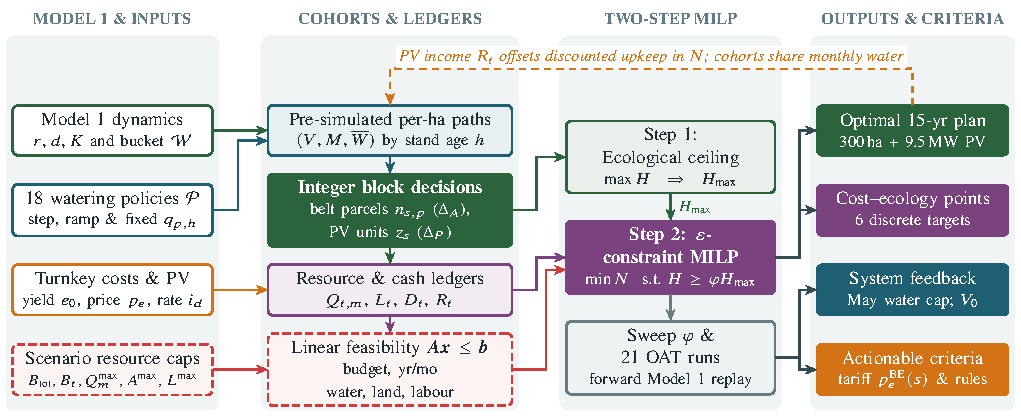
\includegraphics[width=\linewidth]{m2_structure.pdf}
  \caption{Structure of Model~2. Pre-simulated Model~1 cohort paths make all ledgers linear in block decisions.}
  \label{fig:m2-struct}
\end{figure}

\subsection{Model construction}
\paragraph{Cohort idea and ecological benefit.} Tracking only total area $A_t$ cannot distinguish a newly planted shrub ($V_0=2\%$, low water demand) from an older stand ($>12\%$ cover, high summer demand). Instead, we define a \textbf{cohort} $(s,p)$ by its planting year $s\in\{1,\dots,T\}$ and lifetime watering schedule $p\in\mathcal P$ ($18$ schedules: constant $0\text{--}1{,}000$\,mm/yr, step-up or step-down after age $3$ or $5$, and a $100\to300\to600$\,mm/yr ramp). Belt land is chosen in integer blocks $a_{s,p}=\Delta_A n_{s,p}$ ($\Delta_A=50$\,ha) and PV in blocks $y_s=\Delta_P z_s$ ($\Delta_P=100$\,kW), giving active belt stock $A_t=\sum_{s\le t,p}a_{s,p}$, installed PV $P_t^{\mathrm{inst}}=\sum_{s\le t}y_s$, and operating PV $P_t^{\mathrm{op}}=\sum_{s<t}y_s$ (panels built in year $s$ generate from year $s+1$).

Each cohort runs Model~1's daily water bucket $\mathcal W$ (Algorithm~\ref{alg:m1}) under its age-specific quota $q_{p,t-s}$ and updates cover via Eq.~\eqref{eq:m1-veg}. Summing start-of-year cover relative to the local ceiling $K$ across all active cohorts defines the 15-year ecological benefit:
\begin{equation}\label{eq:m2-eco}
H=\sum_{t=1}^{T}\sum_{s\le t,\,p\in\mathcal P}\underbrace{a_{s,p}\,\frac{V_{s,p,t}}{K}}_{\text{effective ha in year }t},\qquad
(M_{s,p,t+1},\,\overline W_{s,p,t})=\mathcal W\!\big(V_{s,p,t},\,M_{s,p,t},\,q_{p,t-s}\big).
\end{equation}
One hectare at $V=K$ for one year scores $1\text{ effective ha}\cdot\text{yr}$. Using start-of-year cover $V_{s,p,t}$ avoids crediting growth before it happens and naturally rewards early planting because desert shrubs take a decade to mature. Because separate strips do not share soil water, running Model~1 \emph{once per schedule} beforehand fixes $V_{s,p,t}$ per hectare, making $H$ strictly linear in $n_{s,p}$.

\paragraph{Investment allocation ratios and PV revenue.} In year $t$, gross spending $D_t$ splits across Task~2's three required uses---construction, O\&M (including water delivery $Q_t$), and PV capital---while operating panels earn electricity revenue $R_t$:
\begin{equation}\label{eq:m2-cash}
D_t=\underbrace{c_b a_t}_{C_t^b:\ \text{build}}+\underbrace{\big(c_m A_t+c_{pm}P_t^{\mathrm{op}}+c_w Q_t\big)}_{C_t^o:\ \text{O\&M + water}}+\underbrace{c_p y_t}_{C_t^p:\ \text{PV}},\quad
R_t=p_e\!\sum_{s<t}y_s e_0(1-d_p)^{t-s-1}.
\end{equation}
Here $a_t=\sum_p a_{t,p}$ is newly treated area, $(f_t^b,f_t^o,f_t^p)=(C_t^b,C_t^o,C_t^p)/D_t$ ($f_t^b+f_t^o+f_t^p=1$ when $D_t>0$) is the annual \textbf{investment allocation ratio}, $e_0$ is first-year net grid yield per kW, $d_p=0.5\%/\text{yr}$ is panel degradation \cite{EN06}, and $p_e$ is the settlement tariff \cite{CN06,EN05}.

\paragraph{System restrictions and explicit trade-off.} Rather than listing separate constraint equations, Figure~\ref{fig:m2-caps} maps how all four resource dimensions---funding, water, land/grid and labour---constrain both new construction flows and cumulative stocks in service. Capital is paid at the start of year $t$ and O\&M/revenue occur at year-end (real discount factor $\delta=(1+i_d)^{-1}$). Instead of inventing a subjective money price for vegetation, we formulate the ecology--cost trade-off via a two-step $\varepsilon$-constraint problem:
\begin{equation}\label{eq:m2-eps}
\min_{\bm n,\bm z}\ N=\sum_{t=1}^{T}\Big[\underbrace{\delta^{t-1}\big(C_t^b+C_t^p\big)}_{\text{year-start capex}}+\underbrace{\delta^{t}\big(C_t^o-R_t\big)}_{\text{year-end O\&M $-$ PV}}\Big]
\;\;\text{s.t.}\;\; H\ge\varphi H_{\max},\ \text{caps in Fig.~\ref{fig:m2-caps}},
\end{equation}
where Step~1 maximises $H$ under the same caps to find the physical ceiling $H_{\max}$, and Step~2 minimises net present cost $N$ for a chosen ecological target share $\varphi\in[0,1]$ ($\varphi=0.60$ in the baseline).

\begin{figure}[!htb]
  \centering
  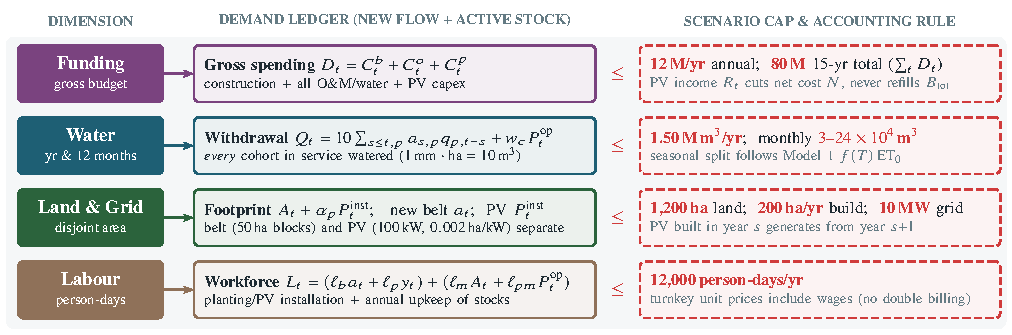
\includegraphics[width=\linewidth]{m2_restrictions.pdf}
  \caption{Resource restrictions and accounting rules of Model~2 across funding, water, land/grid and labour.}
  \label{fig:m2-caps}
\end{figure}

\subsection{Solution approach}
Pre-simulating the 18 schedules in Model~1 converts Eq.~\eqref{eq:m2-eps} into an exact mixed-integer linear programme (MILP) over integer block counts $\bm x=(\bm n,\bm z)$, solved via branch-and-cut (HiGHS, MIP gap tolerance $0.20\%$; Algorithm~\ref{alg:m2-milp}). Every solved plan is independently replayed forward through Model~1 to verify water and cash closure (maximum discrepancy $1.9\times10^{-9}$). Because the problem statement gives no site budget, water quota or tariff, Table~\ref{tab:m2-par} sets an auditable 15-year planning scenario anchored to a 2024 Yutian desert-treatment trial ($52{,}500$\,CNY/ha \cite{REF20}) and literature PV degradation \cite{EN06}.

\begin{algorithm}[!htb]
\caption{Cohort pre-simulation and two-step $\varepsilon$-constraint MILP}\label{alg:m2-milp}
\begin{algorithmic}[1]
\Require Model~1 $(r,d,K,\mathcal W)$, 18-policy library $\mathcal P$, scenario parameters and caps (Table~\ref{tab:m2-par}, Figure~\ref{fig:m2-caps})
\Ensure optimal schedule $\bm x^*$, ceiling $H_{\max}$, trade-off points and sensitivity runs
\State Run Model~1 (Algorithm~\ref{alg:m1}) once per policy $p\in\mathcal P$ from $(V_0,M_0)$ to tabulate per-ha $V_{\mathrm{start}}$ and monthly water
\State Build linear constraint matrix $\bm A\bm x\le\bm b$, ecology vector $\bm h$ (Eq.~\eqref{eq:m2-eco}) and net cost vector $\bm c$ (Eq.~\eqref{eq:m2-eps})
\State \textbf{Step 1:} $H_{\max}\gets\max\{\bm h^\top\bm x:\bm A\bm x\le\bm b,\ \bm x\in\mathbb Z_{\ge0}^m\}$;\quad \textbf{Step 2:} $\bm x^*\gets\arg\min\{\bm c^\top\bm x:\bm A\bm x\le\bm b,\ \bm h^\top\bm x\ge\varphi H_{\max}\}$
\State Sweep $\varphi\in\{0,0.2,\dots,1.0\}$; perturb parameters at fixed $H\ge0.60\,H_{\max}$; replay chosen cohorts in Model~1
\end{algorithmic}
\end{algorithm}

\begin{table}[!htb]
\centering\small
\renewcommand{\arraystretch}{1.06}
\begin{tabularx}{\linewidth}{@{}l X r c l@{}}
\toprule
Symbol & Meaning & Base value & Tested / note & Unit \\
\midrule
$T;\ \Delta_A,\Delta_P$ & horizon; belt block and PV block ($V_0=2\%$, $M_0=37.5$\,mm) & $15;\ 50,\ 100$ & $V_0$: 1--4\% & yr; ha, kW \\
$c_b,\ c_m,\ c_w$ & planting capex \cite{REF20}, belt O\&M, water unit cost & $52{,}500,\ 1{,}500,\ 1.0$ & $c_b\pm25\%$, $c_m\pm50\%$ & CNY (ha, m$^3$) \\
$c_p,\ c_{pm}$ & PV turnkey capex and annual O\&M rate & $3{,}000,\ 50$ & $c_p\pm25\%$ & CNY/kW \\
$e_0,\ p_e,\ d_p$ & 1st-yr PV yield, tariff, degradation \cite{EN06} ($w_c=0.02$\,m$^3$/kW) & $1{,}500,\ 0.30,\ 0.5\%$ & $p_e$: 0.15--0.40 & kWh, CNY, /yr \\
$\ell_b,\ell_m;\ \ell_p,\ell_{pm}$ & belt build/O\&M and PV build/O\&M labour rates & $30,3;\ 0.10,0.01$ & turnkey wages & p-d / (ha, kW) \\
$i_d;\ \varphi$ & real discount rate; baseline ecological target share & $5\%;\ 60\%$ & $\varphi$: 0--100\% & -- \\
\bottomrule
\end{tabularx}
\caption{Key Model~2 scenario parameters (caps shown in Figure~\ref{fig:m2-caps}; Model~1 inputs in Table~\ref{tab:m1-par}).}
\label{tab:m2-par}
\end{table}

\subsection{Results}
\paragraph{Optimal 15-year trajectory and ecology--cost trade-off.} Putting all resources into vegetation gives $H_{\max}=2{,}097.0\text{ effective ha}\cdot\text{yr}$ ($900$\,ha planted, $0$\,MW PV, $N=64.42$\,M\,CNY). At the $\varphi=60\%$ target ($1{,}258.2\text{ effective ha}\cdot\text{yr}$), the optimal schedule (Figure~\ref{fig:m2-plan}) plants $300$\,ha in years 1--2 ($150$\,ha/yr: $250$\,ha on $100\to300$\,mm/yr after age~3, $50$\,ha on $100\to300\to600$\,mm/yr) and installs $9.5$\,MW of PV across years 1--4 ($1.2,1.1,3.7,3.5$\,MW), reaching $H=1{,}264.8\text{ effective ha}\cdot\text{yr}$ at net present cost $N=25.35$\,M\,CNY (MIP gap $0.20\%$).

Three mechanisms shape the four decision trajectories in Figure~\ref{fig:m2-plan}. First, \textbf{front-loading}: years 1--4 use virtually the entire $12$\,M/yr cap, shifting allocation ratios from $66\%$ planting / $30\%$ PV in year~1 to $\sim90\%$ PV in years 3--4 and $100\%$ O\&M thereafter; from year~5, PV revenue ($4.05\text{--}4.25$\,M/yr) covers more than twice annual O\&M and water ($1.83\text{--}1.98$\,M/yr), saving $2.49$\,M ($9.0\%$) over the best no-PV plan ($27.84$\,M). Second, \textbf{age-stepped watering}: giving young seedlings $100$\,mm/yr in ages 1--3 avoids overflowing Model~1's root bucket ($6.6\%$ cheaper than constant quotas), before stepping up as canopy demand grows. Third, \textbf{seasonal bottleneck}: annual water peaks at $1.05\text{ M m}^3\text{/yr}$ ($70\%$ of the annual cap) and labour at $5{,}522$\,p-d ($46\%$), yet \textbf{May water use hits $95\%$ of the monthly cap} in years 8--15---showing that spring delivery, not annual volume, is the true physical constraint.

\begin{figure}[!htb]
  \centering
  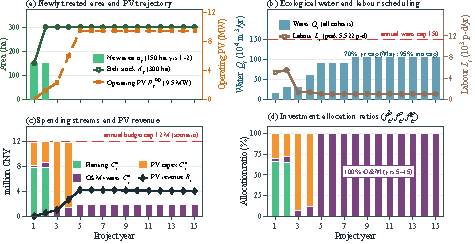
\includegraphics[width=\linewidth]{m2_plan.pdf}
  \caption{Optimal 15-year trajectories of Task~2's four decision groups ($\varphi=60\%$ scenario): (a) newly treated area and operating PV, (b) ecological water and labour scheduling, (c) spending streams vs.\ PV revenue, (d) annual investment allocation ratios.}
  \label{fig:m2-plan}
\end{figure}

Sweeping $\varphi$ from $0\%$ to $100\%$ across six separate MILP solves reveals a sharp cost bend (Figure~\ref{fig:m2-tradeoff}). Up to $\varphi=60\%$, each extra effective $\text{ha}\cdot\text{yr}$ costs $22.6\text{--}26.3$\,k\,CNY while PV stays at $9.5\text{--}10$\,MW. Above $60\%$, marginal cost more than doubles to $36.7$\,k ($80\%$) and $57.1$\,k\,CNY ($100\%$) because higher cover pushes stands into Model~1's diminishing-returns regime and crowds PV out of the $80$\,M gross budget ($10\to5.3\to0$\,MW).

\begin{figure}[!htb]
  \centering
  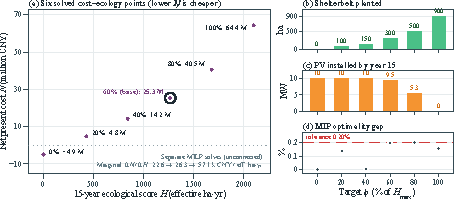
\includegraphics[width=\linewidth]{m2_tradeoff.pdf}
  \caption{Explicit ecology--cost trade-off across six discrete MILP solves (unconnected scenario points; MIP gap $\le0.20\%$).}
  \label{fig:m2-tradeoff}
\end{figure}

\paragraph{Sensitivity of the investment structure.} Holding the ecological requirement fixed at $H\ge1{,}258.2\text{ effective ha}\cdot\text{yr}$ isolates how prices, O\&M and physical assumptions reshape the investment mix (Figure~\ref{fig:m2-sensitivity}):
\begin{enumerate}\setlength{\itemsep}{1pt}\setlength{\parsep}{0pt}
  \item \textbf{PV is all-or-nothing on tariff and capex.} At $0.15$\,CNY/kWh or $3{,}750$\,CNY/kW capex, optimal PV drops to $0$\,MW ($N=27.8$\,M, $+9.8\%$); at $0.40$\,CNY/kWh or $2{,}250$/kW capex, PV hits the $10$\,MW cap and cuts net cost by $30\text{--}44\%$. Forcing PV share $\ge30\%$ has zero effect in the baseline ($41.3\%$ PV share already), showing PV should follow price rather than a fixed quota.
  \item \textbf{O\&M and planting costs shift PV headroom.} Raising O\&M unit rates by $+50\%$ increases $N$ by $+14.8\%$ and squeezes PV down to $5.6$\,MW to preserve maintenance funds; $\pm25\%$ planting capex shifts $N$ by $\pm18\%$.
  \item \textbf{Initial survival $V_0$ outweighs secondary parameters.} Dropping initial cover from $2\%$ to $1\%$ forces $400$\,ha of planting and raises cost $+29.1\%$ ($32.7$\,M), whereas $V_0=4\%$ needs $200$\,ha ($-19.5\%$). Cutting water caps by $20\%$ raises cost $+9.7\%$ ($350$\,ha), while halving labour or refining blocks to $25$\,ha ($-0.22\%$) lies within solver tolerance.
\end{enumerate}

\begin{figure}[!htb]
  \centering
  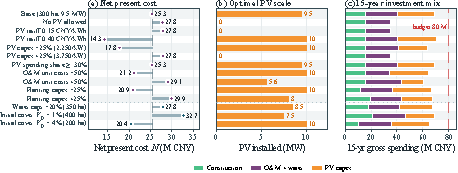
\includegraphics[width=0.95\linewidth]{m2_sensitivity.pdf}
  \caption{Sensitivity of net cost, PV scale and 15-year investment structure at fixed ecological target ($1{,}258.2\text{ effective ha}\cdot\text{yr}$).}
  \label{fig:m2-sensitivity}
\end{figure}

\paragraph{Actionable process criterion.} A standalone $1$\,kW PV unit built in year $s<T$ pays back its capex, O\&M and washing water within the horizon if and only if the tariff exceeds the break-even threshold
\begin{equation}\label{eq:m2-be}
p_e\ge p_e^{\mathrm{BE}}(s)=\frac{c_p+\sum_{t=s+1}^{T}\delta^{t-s+1}\,(c_{pm}+c_w w_c)}{\sum_{t=s+1}^{T}\delta^{t-s+1}\,e_0(1-d_p)^{t-s-1}}.
\end{equation}
\noindent\begin{minipage}[t]{0.54\linewidth}
\vspace{0pt}
In the baseline, $p_e^{\mathrm{BE}}(s)$ rises from $0.253$\,CNY/kWh in year~1 to $0.293$ in year~4 and crosses $0.30$ in year~5 ($0.312$, Figure~\ref{fig:m2-pv}a), matching the MILP's exact build window (years 1--4). This gives four field rules:
\begin{enumerate}\setlength{\topsep}{2pt}\setlength{\itemsep}{0pt}\setlength{\parsep}{0pt}
  \item \textbf{Two-gate PV rule:} install PV in year $s$ only if $p_e\ge p_e^{\mathrm{BE}}(s)$ \emph{and} budget slack remains after planting.
  \item \textbf{Plant in years 1--2:} front-load belt construction so shrubs accrue cover across the full horizon.
  \item \textbf{Ramp water by stand age:} supply $100$\,mm/yr in ages 1--3, step to $300$\,mm/yr at age~4, and $600$\,mm/yr (age $8+$) on core strips.
  \item \textbf{Size for May \& audit $V_0$:} dispatch against May--July water caps, secure $V_0\ge2\%$ via pilot plots, and target the $40\text{--}60\%$ cost knee.
\end{enumerate}
\end{minipage}\hfill
\begin{minipage}[t]{0.43\linewidth}
\vspace{0pt}\raggedleft
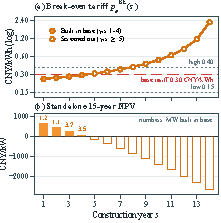
\includegraphics[width=0.90\linewidth]{m2_pv_screen.pdf}
\captionof{figure}{Standalone PV entry screen by build year $s$ (excludes resource opportunity cost).}
\label{fig:m2-pv}
\end{minipage}

\paragraph{Summary.} Cohort pre-simulation embeds Model~1's water--cover physics into a linear multi-year allocation model. Front-loading belt planting in years 1--2, stepping water up with stand age, and building PV only while $p_e\ge p_e^{\mathrm{BE}}(s)$ cuts net cost by $9\%$ and funds long-term upkeep, while identifying May water delivery and seedling survival $V_0$ as the critical vulnerabilities tested under stochastic disasters in Model~3.
